\section{Deployment Diagram}\label{sec:sprint2-deploymentdia}
\autoref{sec:sprint1-architecture} introduced the different components of the system in \autoref{fig:architecture}.
In order to further elaborate on the different components, a deployment diagram is constructed.
\begin{figure}[H]
    \centering
    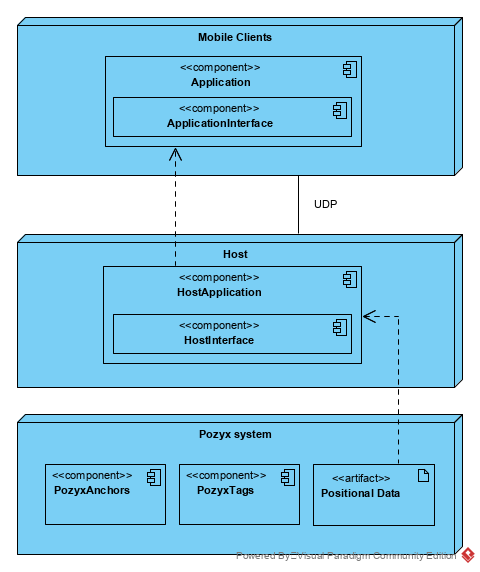
\includegraphics[width=0.6\linewidth]{Deploymentdiagram.png}
    \caption{A deployment diagram for the system.}
    \label{fig:sprint2-deployment}
\end{figure}
\noindent
A deployed system will contain three nodes:
\begin{itemize}
    \item Pozyx system
    \item Host
    \item Mobile Clients
\end{itemize}
Nodes are represented by cubes, and are entities executing components.
The Pozyx system node contains two components.
These are the anchors and the tags needed to generate positioning data with the Pozyx hardware.
The system contains multiples of each.
These Pozyx components generate artifacts in terms of positional data for the location of the players and the ball.
The host node is dependent on the positional data artifact, the component receives the positional data and transforms it for communication.
The host application component also contains an interface component, which is the interface that the person using the host component will interact with, in the form of a terminal application for the early version of the system.
The host node is associated with the clients through a UDP connection in order to communicate the positional data.
As such, the mobile client application component is dependent on the host application component.
The mobile clients also contain interface components, which is how the users interact with that part of the system.
This interface is the virtual playing field generated in Unity, that the users see in the headset.
